\problemname{Brandpost}
\noindent
Brandmannen Robert har jobbat som brandman i över 20 år och älskar sitt jobb. 
Efter en lång promenad i metropolen M (tidigare känd som Stockholm) fick Robert ett samtal på sin telefon från hans hydrofoba chef som beordrade honom att komma in till brandstationen nu på en gång.
Robert anlände nyss till den mest syd-västra fyrvägskorsningen i metropolen M och bestämmer sig för att bege sig direkt till brandstationen, 
men tydligen har flera av brandposterna i metropolen M börjat läcka vatten och svämmar över gatorna! Åh nej! 
Detta är särskilt allvarligt eftersom Roberts hydrofoba chef på brandstationen är stenhård med att inte ha vatten nära sig, 
så att dyka upp dyngsur till jobbet efter att ha stött på flera av de läckande brandposterna kommer få Robert avskedad. 
Robert vill åtminstone arbeta som brandman i 20 år till, 
så hjälp Robert att minimera hur blöt han blir!

Metropolen M består av ett rutnät med storlek $W \times H$,
där varje fyrvägskorsning är en ruta i rutnätet, och går att nå från de fyra intilliggande korsningarna i varje
väderstreck: norr, öster, söder och väster. Robert anlände nyss till fyrvägskorsningen längst
syd-väst i rutnätet, vid ruta $(1,1)$. Robert vill nå brandstationen längst nord-öst i rutnätet,
vid ruta $(W,H)$. Det tar exakt 1 minut att springa från en fyrvägskorsning till en annan
intilliggande korsning. Det är garanterat att brandstationen inte ligger vid $(1,1)$. 

Vidare har $N$ fyrvägskorsningar en läckande brandpost i sig, som kan befinna sig på alla rutor i rutnätet, inklusive där Robert börjar ifrån $(1,1)$, och vid brandstationen $(W,H)$. 
Robert anländer till ruta $(1,1)$ vid minut 0, och varje läckande brandpost har läckt en enhet vatten till korsningen
den sitter vid. För varje minut $t$ som passerar kommer varje läckande brandpost
att läcka en extra enhet vatten till alla korsningar inom en viss avstånd från den
läckande brandposten. Mer specifikt innebär det att alla rutor $(x,y)$ som uppfyller det följande olikheten vid minut $t$ kommer att öka med 
en enhet vatten av brandposten som ligger vid $(x_b,y_b)$:
$$
|x-x_b|+|y-y_b|\le t.
$$

Låt oss kalla antalet enheter vatten som finns vid en viss ruta för $v_t$ vid minut $t$. 
När Robert anländer till en fyrvägskorsning vid minut $t$ kommer Roberts kläder bli våta av allt vatten 
som finns vid den korsningen från läckande brandposter, alltså $v_t$ enheter vatten.

Vad är det minsta totala antalet vattenenheter som Robert behöver gå igenom på väg till brandstationen?

\begin{centering}
  \begin{figure}[h]
    \centering
  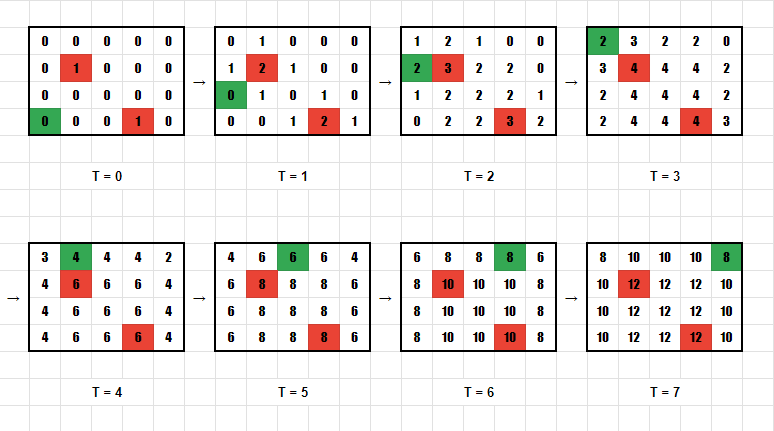
\includegraphics[width=1\textwidth]{brandpostSample1.png}
    \caption{Illustration av exempelfall 1, där det gröna är Roberts position, och de röda är brandposternas position. Det minsta antalet enheter vatten i detta fall är $0+0+2+2+4+6+8+8=30$.}
    \label{fig:brandpost}
  \end{figure}
\end{centering}

\section*{Indata}
Den första raden i indatan innehåller tre heltal, $W$, $H$ ($1 \le W,H \le 1000$) och $N$ ($1 \le N \le min(20000,W \cdot H)$), 
där $W$ och $H$ är bredden respektive höjden på rutnätet, och $N$ är antalet läckande brandpost som finns i rutnätet.

Därefter följer $N$ rader, där varje rad består av två heltal $x_i$ ($1 \le x_i \le W$) och $y_i$ ($1 \le y_i \le H$), 
och $(x_i,y_i)$ är koordinaterna för den $i$:te läckande brandposten i rutnätet. 
Det är garanterat att alla brandposter har olika koordinater, alltså att $(x_i,y_i) \neq (x_j,y_j)$ för alla index $1 \le i < j \le n$.

\section*{Utdata}
Skriv ut ett heltal, det minsta totala antalet vattenenheter som Robert behöver gå igenom på väg till brandstationen.

\section*{Poängsättning}
Din lösning kommer att testas på en mängd testfallsgrupper.
För att få poäng för en grupp så måste du klara alla testfall i gruppen.

\noindent
\begin{tabular}{| l | l | p{12cm} |}
  \hline
  \textbf{Grupp} & \textbf{Poäng} & \textbf{Gränser} \\ \hline
  $1$    & $10$       & $W,H \le 10$, $N=1$ och den enda brandposten finns vid $(1,1)$. \\ \hline
  $2$    & $15$       & $W,H,N \le 50$ \\ \hline
  $3$    & $17$       & $W,H \le 100$, $N\le 200$\\ \hline
  $4$    & $27$       & $W,H \le 150$ \\ \hline
  $5$    & $31$       & Inga ytterligare begränsningar. \\ \hline
\end{tabular}

